\documentclass[a4paper,10pt]{report}
\usepackage[T1]{fontenc}
\usepackage[utf8]{inputenc}
\usepackage{lmodern}
\usepackage[francais]{babel}
\usepackage{amsmath} % math
\usepackage{amssymb} % math
\usepackage{gensymb} % math
\usepackage{graphicx} % images
% \usepackage{qtree}    % dessiner des arbres %% => texlive-humanities
\usepackage{url}
\urlstyle{sf}
\usepackage{multicol} % for multicolonm
\usepackage{subfig} % for subfigure
\usepackage[usenames]{color}
\usepackage[french]{varioref} % \vpageref
\usepackage[top=2.5cm, bottom=2.5cm, left=2.5cm, right=2.5cm]{geometry}
\definecolor{codeBlue}{rgb}{0,0,1}
\definecolor{webred}{rgb}{0.5,0,0}
\definecolor{codeGreen}{rgb}{0,0.5,0}
\definecolor{codeGrey}{rgb}{0.6,0.6,0.6}
\definecolor{webdarkblue}{rgb}{0,0,0.4}
\definecolor{webgreen}{rgb}{0,0.3,0}
\definecolor{webblue}{rgb}{0,0,0.8}
\definecolor{orange}{rgb}{0.7,0.1,0.1}
\usepackage{caption}
\renewcommand{\familydefault}{\sfdefault}
\usepackage{listings}        % Pour l'insersion de fichiers de codes sources.
\lstset{
      language=Java,
      flexiblecolumns=true,
      numbers=left,
      stepnumber=1,
      numberstyle=\ttfamily\tiny,
      keywordstyle=\ttfamily\textcolor{blue},
      stringstyle=\ttfamily\textcolor{red},
      commentstyle=\ttfamily\textcolor{green},
      breaklines=true,
      extendedchars=true,
      basicstyle=\ttfamily\scriptsize,
      showstringspaces=false
    }
%%%%%%%%%%%%%%%%%%%%
\title{Bouboule - Manual}
\author{Matthieu \textsc{Baerts} \and Baptiste \textsc{Remy} \and Nicolas \textsc{Van Wallendael} \and Hélène \textsc{Verhaeghe}}
    \date{\today}
\begin{document}
\maketitle

\section*{Description of the different views}

\begin{figure} [h!]
	\centering
	\subfloat[Main menu]{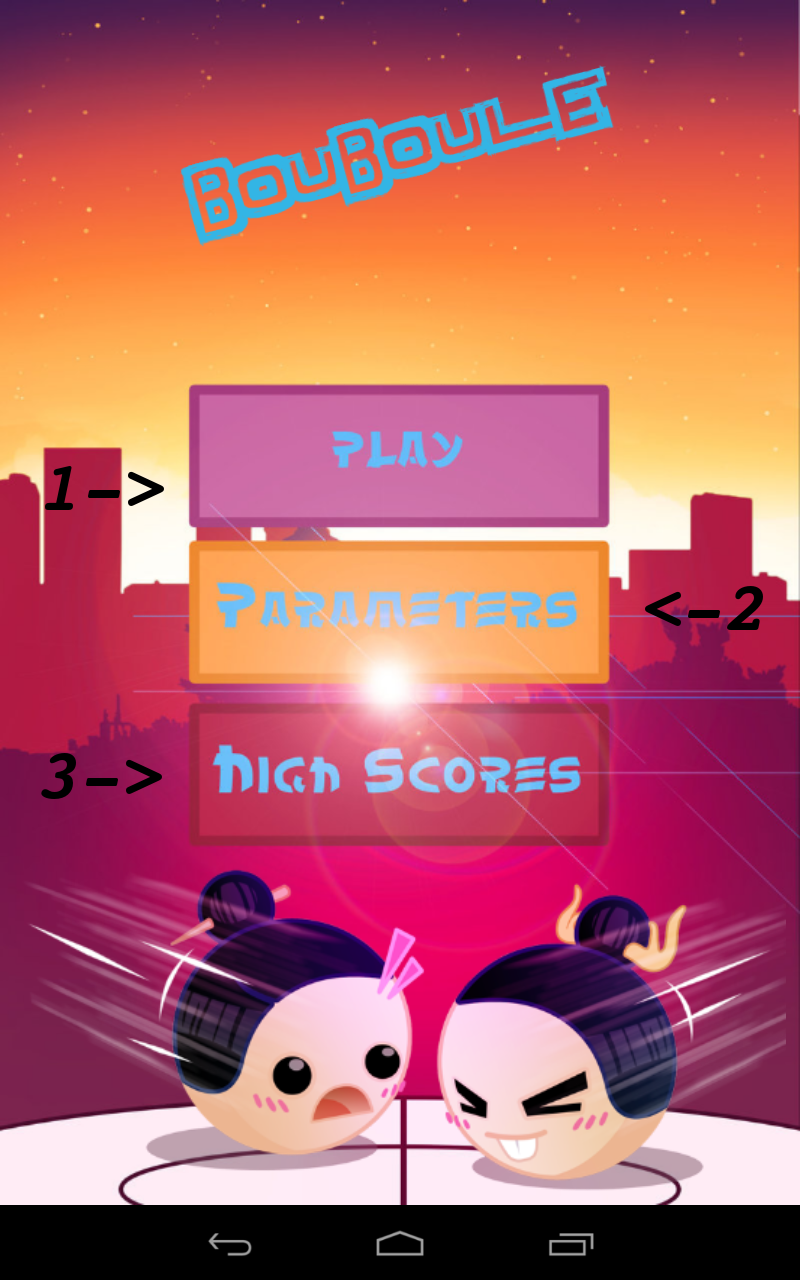
\includegraphics[scale=0.15]{1_Menu.png}}
	\subfloat[World selector]{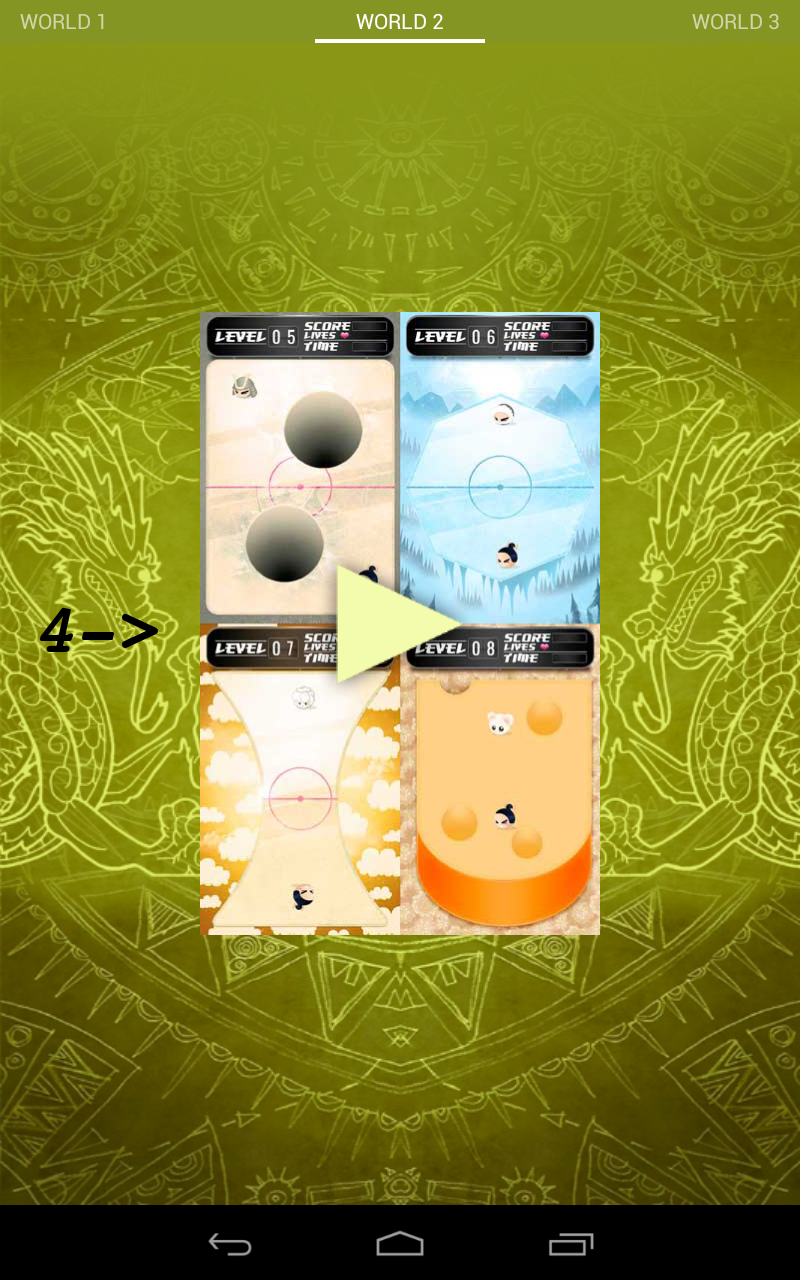
\includegraphics[scale=0.15]{2_WorldSelector.png}}
	\subfloat[Game]{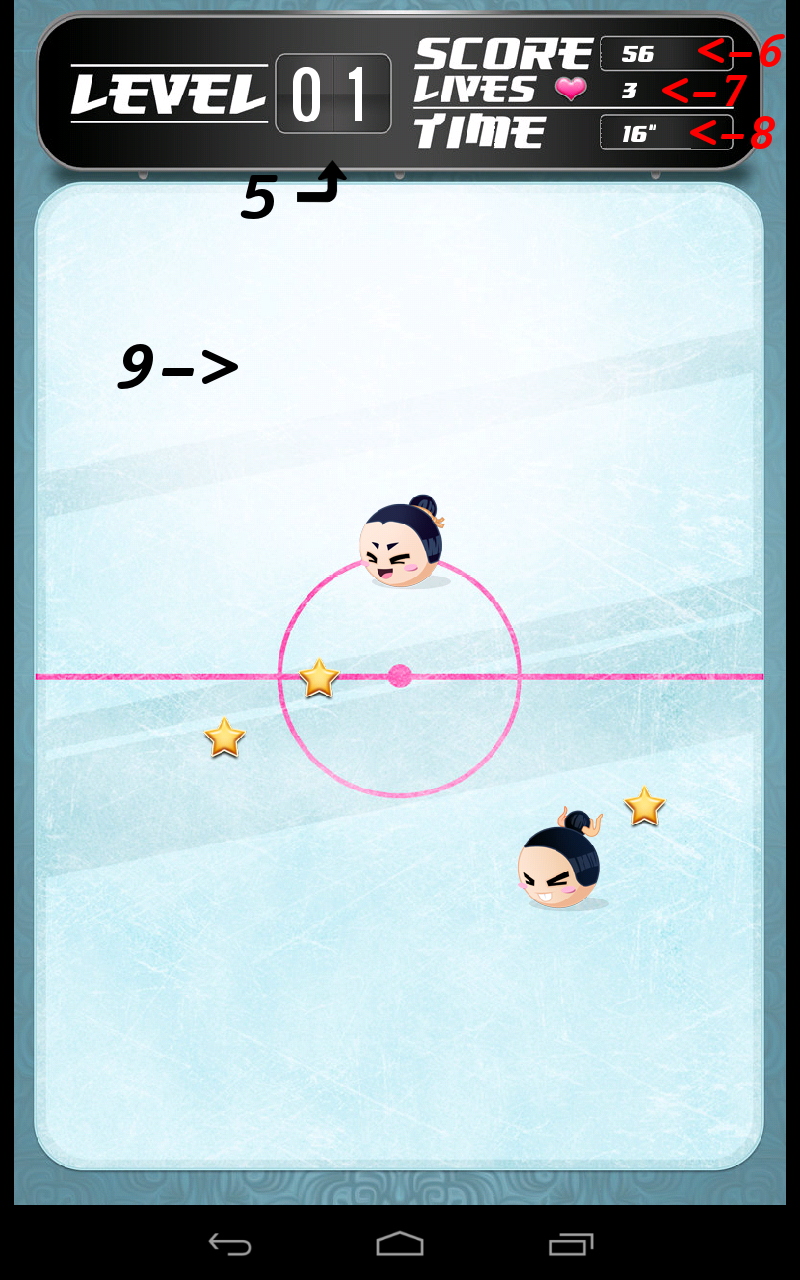
\includegraphics[scale=0.15]{3_Game.png}}\\
	\subfloat[Winning screen]{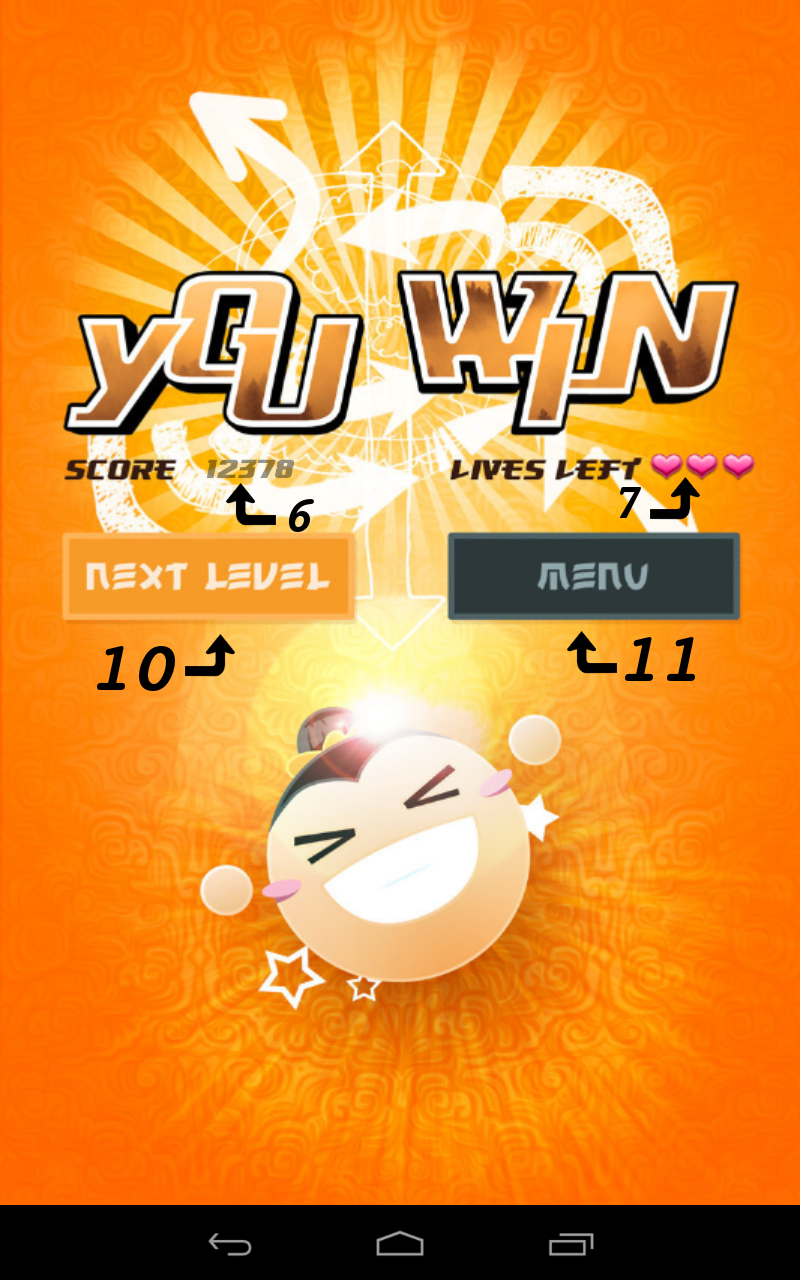
\includegraphics[scale=0.15]{4_Win.png}}
	\subfloat[Losing screen]{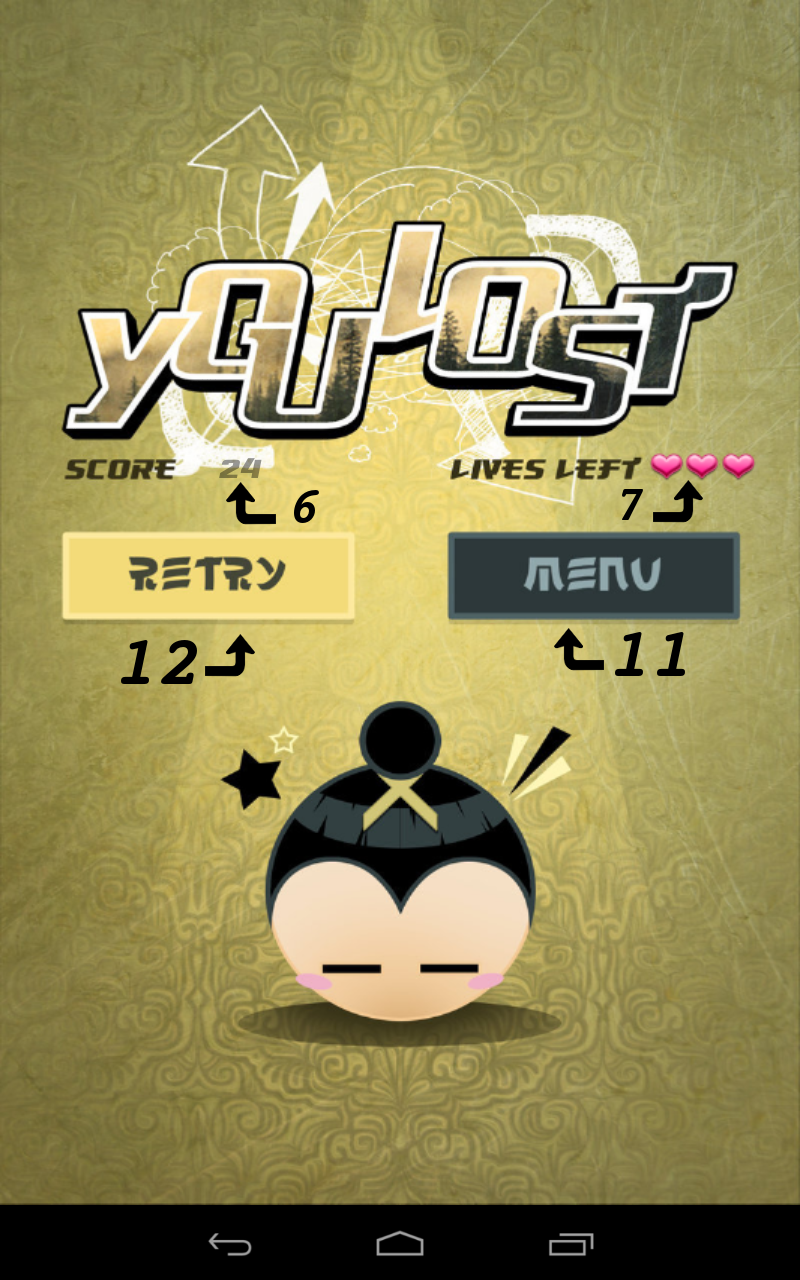
\includegraphics[scale=0.15]{5_Lost.png}}
	\subfloat[Game over screen]{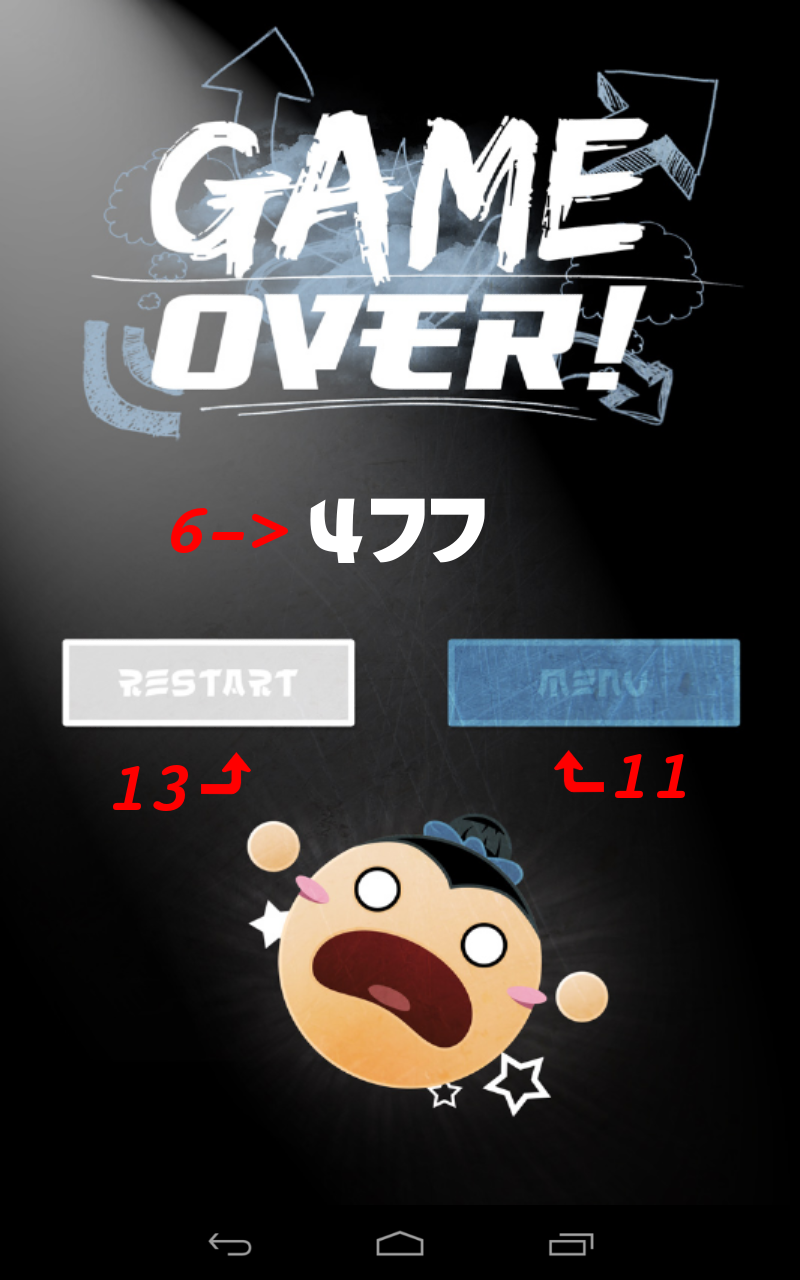
\includegraphics[scale=0.15]{6_GameOver.png}}\\
	\subfloat[Settings menu]{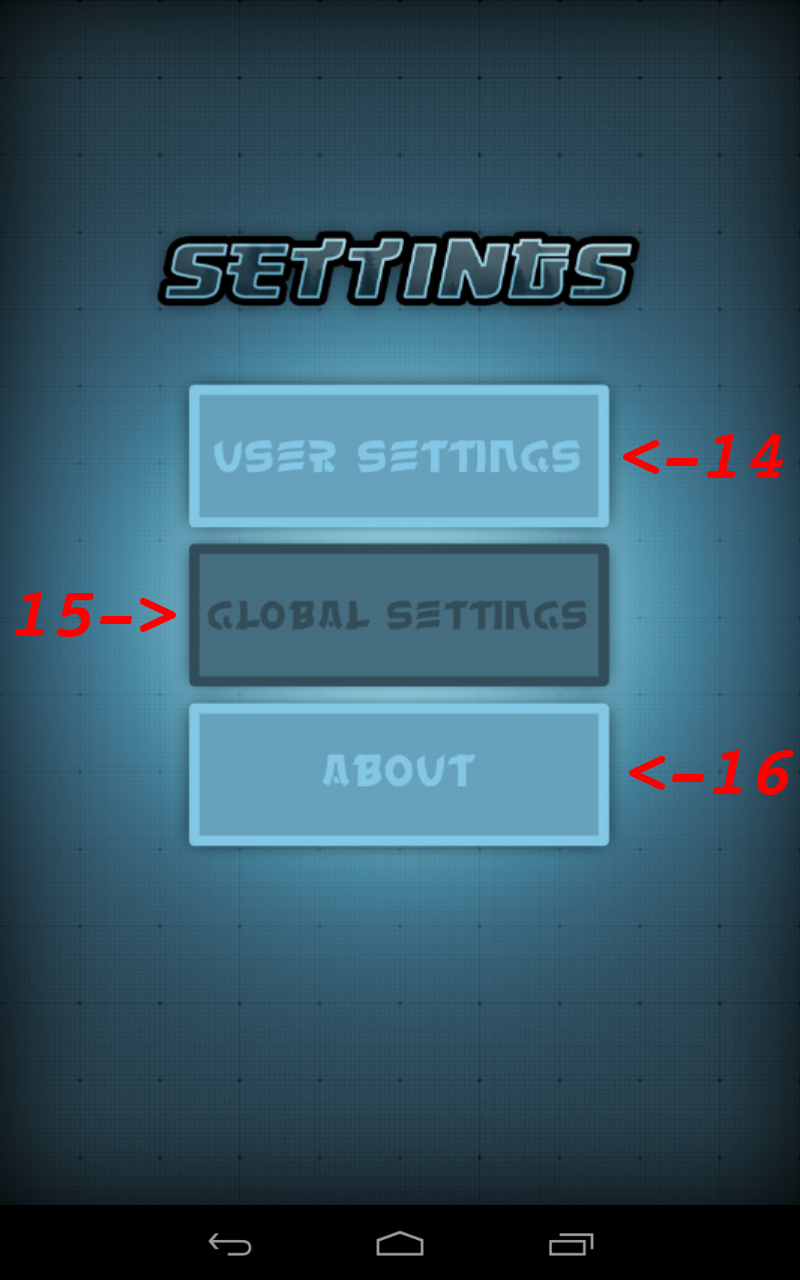
\includegraphics[scale=0.15]{7_Settings.png}}
	\subfloat[User settings menu]{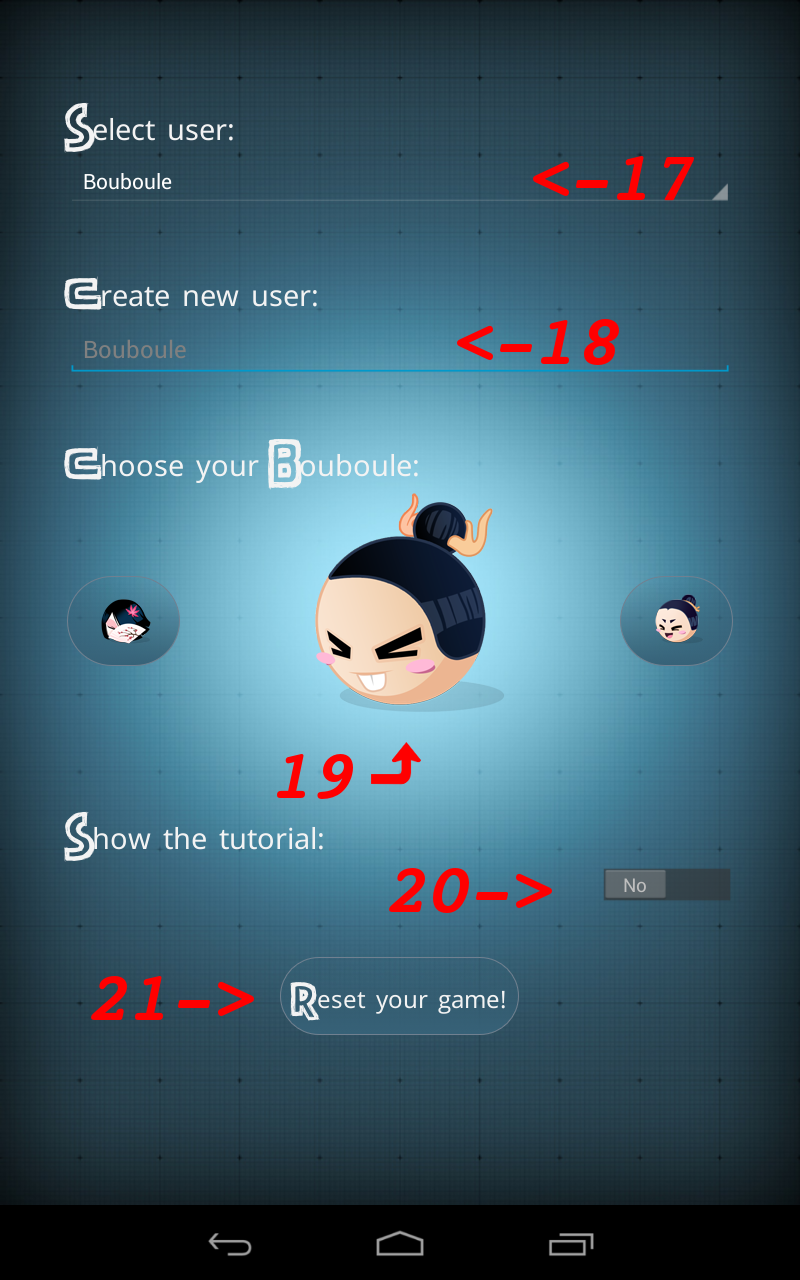
\includegraphics[scale=0.15]{8_UserSettings.png}}
	\subfloat[Global settings menu]{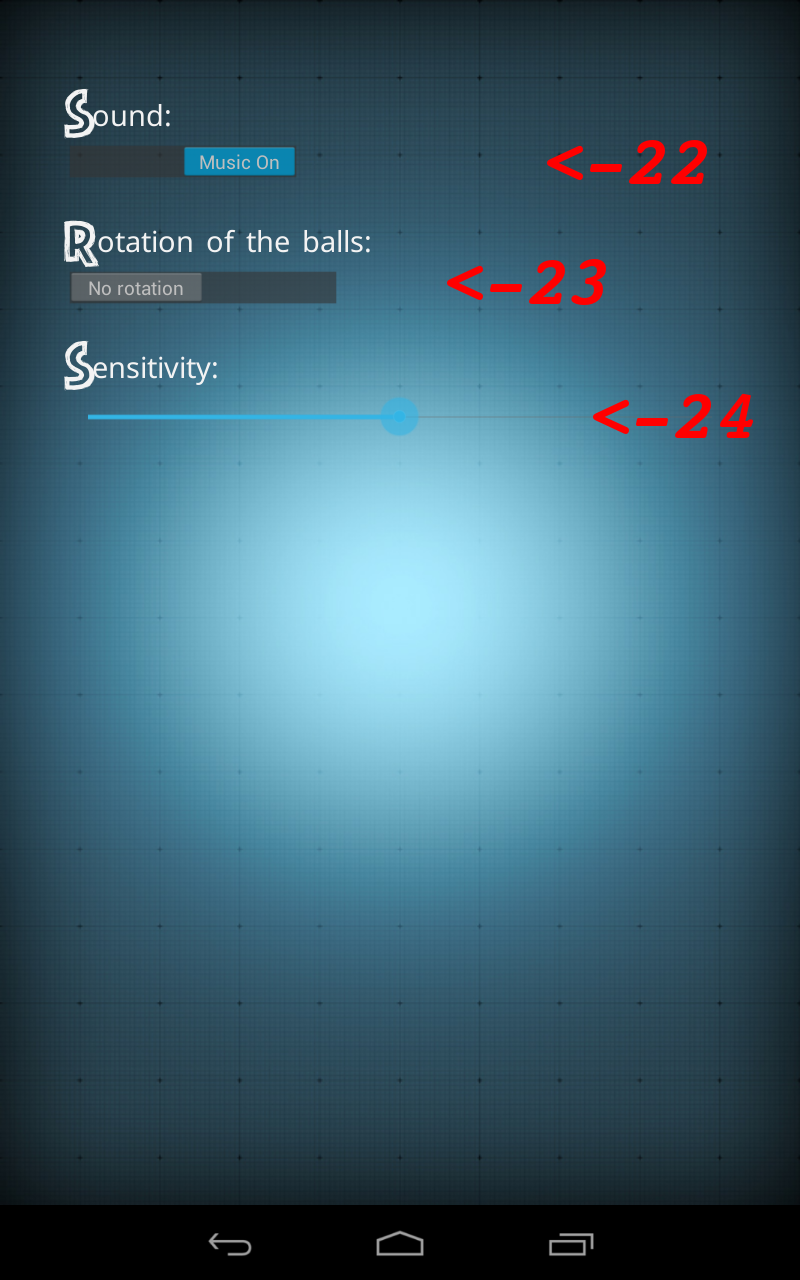
\includegraphics[scale=0.15]{9_GlobalSettings.png}}
\end{figure}


\begin{multicols}{3}
\begin{enumerate}
\item Play button
\item Settings button
\item Highscore button
\item World selector
\item Level
\item Score
\item Remaining lives
\item Remaining time
\item Gameboard
\item Next level button
\item Menu button
\item Retry button
\item Restart button
\item User settings button
\item Global settings button
\item About button
\item User selector
\item New user creator
\item Bouboule selector
\item Tutorial switch
\item Reset game button
\item Sound switch
\item Rotation switch
\item Sensitivity selector
\end{enumerate}
\end{multicols}


\section*{How to?}

	\subsection*{How to create a new user profile?}
First, on the menu, goes to the settings menu (2). Then, goes to the user section (14). Now you are in the user setting section. Write your player name in the new user creator (18), then validate it on the enter button on the keyboard. Your new profile is created! You can see it on the user selector (17) where the current player is always on top.

!! Warning !! : you can't chose already taken names, names containing specials characters or any special combination of characters that are invalid files names. But don't worry! a toast will appear if you are using a wrong name.

Now you can back to the main menu to play or stay in this menu to personnalise your profile.

	\subsection*{How to change current user profile?}
	
First, goes to the user setting menu (from main menu go first in the settings (2), then in the user settings (14)). Then, click on the user selector (17). The list of the différents potential users is display. Chose the one you want by clicking on it. Your profile is selected! You can see it on the user selector (17) where the current player is always on top.

Now you have selected your profile, you can go back to the main menu to play or stay in this menu to personnalise your profile.

	\subsection*{How to personalise my profile?}

First, goes to the user setting menu (from main menu go first in the settings (2), then in the user settings (14)). Make sure the selected user is the one you want to personalise by watching the user selector (17). If the user shown is yours then it is alright otherwise change the current user. You are able to do several changes.

		\subsubsection*{Change the character}

With the Bouboule selector (19) you are able to change the Bouboule you are playing. You can only embody Bouboule you have already defeat so if you can't switch go play and win games to win skins.

		\subsubsection*{Tutoriel}

A little tutoriel is display on the screen the first time you play the first level. If you want to see it again just switch the tutorial switch (20).

!! Warning !! : If you ask to have the tutorial again, your current save game will be reseted.

		\subsubsection*{Reset}
		
If you want to reset your save game just press the resset button (21) and it will be done.

	\subsection*{How to play?}

In the main menu, click on play (1). You have now access to the world selector (4). Just swipe between world to chose the one you want to go and click on it to begni the game. If you don't access to the world selector by pressing the play button (1), but, instead, you arrive in a game, it's mean that you have a current save game. It restart where you where stopped.

When you are playing just tilt the device to control the Bouboule. And don't forget, the aim is to set the other outside the arena, but pay attention, don't go outside yourself.

During the game, you can see witch level you are playing (5), what is your current score (6), how many live you remains (7) and how much time do you have still to finish the level (8).

When you win a battle, you arrive at the winning screen where you can see the score (6) and your remaining lives (7). You can now go to the next level (10) or go back to the main menu (11) to quit the game, to change your bouboule with the new one won, or to do whatever you want.

If you lose your battle, you arrive on the losing screen. You can see your score (6) and your remaining lives (7). You can either retry the battle (12) or go the main menu (11).

When you lose and you don't have remaining lives you go to the game over sceen. Your score is display (6). If it is high enough it will be added to the highscore (you can view it went you are on the main menu by clicking on the highscore button (3)). At this point you can restart a game (13) (you will land on the world selector (4)) or go the main menu (11).

	\subsection*{How to pause the game?}

	When you are in game, just press back and you will be on pause. You can then chose to resume the game, go the the main menu or quit the application. Your current game progression will be saved and resume the next time you will play (unless you reset the game).
	
	\subsection*{Some other settings}

	If you go in the global settings menu (form the main menu, go to settings (2) and then to global settings (15)), you can also chose if you want music (22) or if you want that the bouboule rotate (23). You can also move the sensibility of the device (24).







\end{document}
